
\section{Neural-Networks}
\label{sec:neural_networks}

	In this section we will see how neural-network manage to solve classification tasks. As a reminder, a classification problem aims at identifying the sub-populations of a set belonging to a class. More specifically : if we are given a set of inputs $X$ and outputs $Y$. where $x^i$ denotes a sample from the set $X$ and $y^i$ its class. Then, the aim of classification is to predict the class a new sample given the knowledge based on the $x^i$'s.

	Artificial neural-networks are a family of statistical learning algorithms. They are inspired from the human brain structure : nowadays, we believe the brain has a network of neurons triggering signals over its dendrite and propagated to other neurons through a synapse interface. Network of artificial neurons mimics these properties.

	In this section, we will first introduce what are the artificial neurons and how do we aggregate them to make neural-networks. After we've seen this, we will see how to train these networks: what is a cost and how do we reduce the error made by these networks.


	\subsection{Artificial neuron and Perceptron}
	\label{sec:Artificial_neurons}
		First, the neurons. The first neuron we mention here is the \textbf{Perceptron}. It was described by Rosenblatt in 1958 \cite{rosenblatt1958perceptron} and was one of the first artificial neuron introduced in the literature. This neuron takes as an input multiple binary values to which it apply weights. Once multiplied, these \textit{weighted inputs} are summed-up. If the sum is lower than zero, the neuron outputs zero. Otherwise, the neuron outputs one. A schema of an artificial neuron is given on \Fref{fig:perceptron}.

		Formally: given an input vector $x$ of size $m$ where $x_i$ is the $i$th element of $x$, the Perceptron defines a weight vector $w$ with same shape as the input vector $x$ and a bias term $b$. Then its transfer function is :

		$$ \text{Perceptron}(x) = \begin{cases}1 & \text{if } \sum_{j=0}^m (w_j \times x_j) + b > 0\\0 & \text{otherwise}\end{cases} $$

		In a vector notation this becomes 

		$$ \text{Perceptron}(x) = \begin{cases}1 & \text{if } w^T \cdot x +b > 0\\0 & \text{otherwise}\end{cases} $$

		\begin{figure}
			\centering
			\def\layersep{1.5cm}
			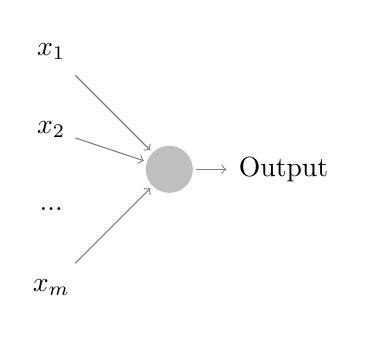
\begin{tikzpicture}[shorten >=1pt,->,draw=black!50, node distance=\layersep]
				\tikzstyle{tata}=[,minimum size=17pt,inner sep=0pt]
			    \tikzstyle{neuron}=[circle,fill=black!25,minimum size=17pt,inner sep=0pt]
			    \tikzstyle{output neuron}=[neuron, fill=red!50];

			    % Input neurons
			    \node[tata] (x1) at (0,-1 cm) {$x_1$};
			    \node[tata] (x2) at (0,-2 cm) {$x_2$};
			    \node[tata] (x3) at (0,-3 cm) {...};
			    \node[tata] (x4) at (0,-4 cm) {$x_m$};
			    
			    % Draw the output layer node
			    \node[neuron,pin={[pin edge={->}]right:Output}] (O) at (\layersep,-2.5) {};

			    % Connect every node in the hidden layer with the output layer
			    \path (x1) edge (O);
			    \path (x2) edge (O);
			    \path (x4) edge (O);

			\end{tikzpicture}
			\label{fig:perceptron}
			\caption{Model of an artificial neuron}
		\end{figure}

		Nowadays we use other types of neurons. As the Perceptron, these neurons consider a weighted sum of their inputs plus a bias term. Now, their activation function is different and their outputs are real valued. We present two of the well known neurons:
		\begin{itemize}
			\item The \textbf{sigmoid neuron} is defined by a smooth threshold function :
			$$ \sigma(x) = \frac{1}{1 + e^{-x}} $$
			\item The \textbf{Regression Logistic Unit} (ReLU) is a neuron which activation function is equal to zero for any negative inputs and equal to its input otherwise.
			$$ \text{ReLU}(x) = \begin{cases} ?? & \text{if } w \cdot x + b > 0 \\0 & \text{otherwise}\end{cases} $$
		\end{itemize}


	\subsection{Neural-network}
		Now that we have neurons, we need a network of them to compose an architecture similar to the brain. The networks we are going to work with are called \textbf{feed-forward} neural-networks. They are the most common ones in the literature. \Fref{fig:feed_forward} is a representation of a two-hidden-layer feed-forward neural-network. As you can see, this model consist of groups of neurons. We denote as layer the group of neurons belonging to the same deepness in the model. Therefore, all the neurons visible on the left in our model, compose the first layer of neurons. It's the input layer. The following layers are called the hidden layers and the last one is the output layer. Some variations exists of this definition, for instance, some outputs of the model might be placed at the same level as some hidden layer.

		Our simple example is also a feed-forward neural-network. It has an input layer fully connected to a hidden layer, which is also fully connected to the output layer. As drawn on the schema with the directions of the arrows, the signal propagates from left to right, from the inputs to the outputs. Because of these two reasons (layers fully connected and single direction signal propagation) our simple example is a feed-forward neural-network.		

		\begin{figure}
			\centering
			\def\layersep{1.5cm}
			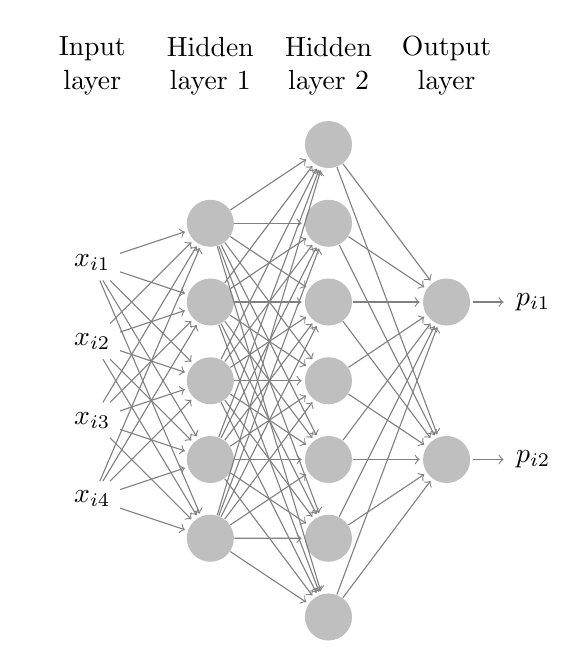
\begin{tikzpicture}[shorten >=1pt,->,draw=black!50, node distance=\layersep]
			    \tikzstyle{every pin edge}=[<-,shorten <=1pt]
			    \tikzstyle{neuron}=[circle,fill=black!25,minimum size=17pt,inner sep=0pt]
			    \tikzstyle{annot} = [text width=4em, text centered]


			    %%%%%%%%%%%%%%%%%%%%%%%%%%%%%%%%%%%%%%%%%%%% 
			    %%% DRAW THE NODES
			    %%%%%%%%%%%%%%%%%%%%%%%%%%%%%%%%%%%%%%%%%%%%
			    \foreach \name / \y in {1,...,4}
			        \node[] (I-\name) at (0,-\y) {$x_{i\y}$};

			    \foreach \name / \y in {1,...,5}
			        \path[yshift=0.5cm] node[neuron] (H1-\name) at (\layersep,-\y cm) {};

				\foreach \name / \y in {1,...,7}
			        \path[yshift=1.5cm] node[neuron] (H2-\name) at (\layersep*2,-\y cm) {};   

		       	
			    \node[neuron,pin={[pin edge={->}]right:$p_{i1}$}, right of=H2-3] (O-1) {};
			    \node[neuron,pin={[pin edge={->}]right:$p_{i2}$}, right of=H2-5] (O-2) {};

			    %%%%%%%%%%%%%%%%%%%%%%%%%%%%%%%%%%%%%%%%%%%% 
			    %%% DRAW THE PATHS
			    %%%%%%%%%%%%%%%%%%%%%%%%%%%%%%%%%%%%%%%%%%%%
			    \foreach \source in {1,...,4}
			        \foreach \dest in {1,...,5}
			            \path (I-\source) edge (H1-\dest);

			    \foreach \source in {1,...,5}
			        \foreach \dest in {1,...,7}
			            \path (H1-\source) edge (H2-\dest);

			    \foreach \source in {1,...,7}
			    	\foreach \dest in {1,...,2}
				        \path (H2-\source) edge (O-\dest);

			    % Annotate the layers
			    \node[annot,above of=H2-1, node distance=1cm] (hl) {Hidden layer 2};
			    \node[annot,left of=hl] (hl1) {Hidden layer 1};
			    \node[annot,left of=hl1] {Input layer};
			    \node[annot,right of=hl] {Output layer};
			\end{tikzpicture}
			\label{fig:feed_forward}
			\caption{Feed-forward neural-network with two hidden layers}
		\end{figure}


		It's good to mention that other types of network exits such as the \textbf{recurrent networks}. In these networks, there is directed cycles on the graph which means that a neuron can depends on its own output. This model is considered to be closer to the brain structure but the challenge on training these models isn't state of the art. We won't work on these models.

		\textbf{Symmetrically connected} networks is an other types of network, they are called the "Boltzmann machines". They are symmetrical in the sense that connections between neurons exists in the two directions and the weight on this connections is the same in both directions. Here again, we won't work on these models.


	\subsection{Forward propagation}
		

	

	\subsection{Cost function}
		Once we have build our model, we consider a cost function, also called "loss function". This cost function define how good is the model considering an evaluation criterion. In the case of classification, we want to evaluate how good the prediction is doing towards the true output.
		The most famous cost functions in neural-network classification are the squared error and the cross entropy (also called the "negative log-likelihood"). They are defined as follows for a given sample $i$ and output $j$.
		\begin{itemize}
			\item Squared error : $$ l(p_{ij},y_{ij}) = \norm{y_{ij} - p_{ij}}_2^2 $$
			\item Cross entropy : $$ l(p_{ij},y_{ij}) = -\ln(p_{ij})_{y_{ij}}  ??? $$ 
		\end{itemize}

		Lets take an example. Consider the model presented on \fref{fig:feed_forward}. To this model, we input $x_i$ and propagate the signal until the last layer. This last layer gives us the prediction $p_i = [0.9,0.15]$. Given with $x_i$ we had its true prediction $y_i = [1,0]$. We have everything to compute the two loss functions described earlier : 
		\begin{itemize}
			\item Squared error : $$ l(p_{ij},y_{ij}) =  .1^2 + .15^2 $$
			\item Cross entropy : $$ l(p_{ij},y_{ij}) = -\ln(.1)  $$
		\end{itemize}


	\subsection{Back-propagation}
		Back propagation is the 


		\vspace{1em}
		\textbf{Notation : }\\


	\subsection{Gradient descent}

	\section{Multi-layer neural-network}
		The softmax network we've been previoulsy working with is a single-layer  neural-network, composed by softmax units (or softmax neurons). We are now going to work on a network containing more layers. Instead of forwarding our input data $X$ into the softmax units, we will input them into Rectified Linear Units (ReLU).

		\subsection{Rectifiect Linear Units}
		A ReLU is similar to a perceptron but it has a different transfert function. As the perceptron, it has many inputs an one output. The output is a function of the sum of the weighted inputs. This function is defined as :
		$$ h_t(x) =  $$
		All together, the ReLU outputs :
		$$ \text{ReLU}(X) =  (W^Tx_i) $$

		\subsection{Defining the multi-layer net}
		The Multi-layer neural-network we first study has two layers of composed by 500 ReLU neuron each and an output layer of softmax units. 